\section{Additional GPU Validation Records}\label{app:gpu}
The new records comprise three seeds per dataset for ARM and for each
ARD variance-update setting. Gate bins in Table~\ref{tab:armgates} and
the individual constraint trajectories in Figure~\ref{fig:armconstraints}
show why a thresholded dimension count is insufficient to diagnose
successful pruning. In particular, dSprites does not approach a decisive
binary gate configuration or a satisfied constraint.
@@table52:arm_gates@@

\begin{figure}[!htbp]
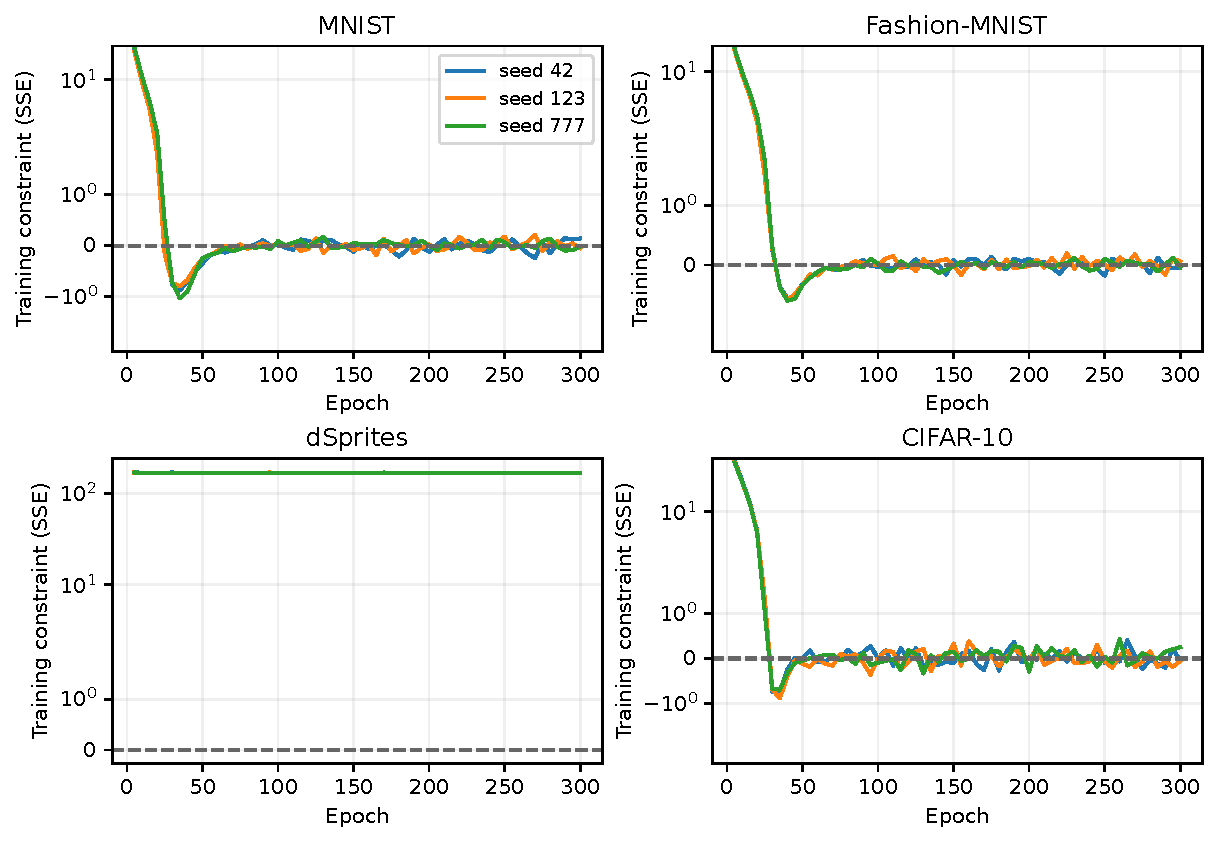
\includegraphics[width=\textwidth]{results/figures/MAKE52/arm_constraints.pdf}
\caption{Moving-average stochastic training constraint for each new ARM
seed, recorded every five epochs. Zero is the constraint boundary;
negative values satisfy it. A symmetric logarithmic vertical scale
accommodates large positive violations and negative values. These
trajectories are distinct from deterministic validation-target attainment.}
\label{fig:armconstraints}
\end{figure}

Figures~\ref{fig:armcurves} and~\ref{fig:ardcurves} report evaluation-mode
reconstruction curves for all four datasets. They describe the supplied
300-epoch runs; a visually flat curve does not certify an optimum.
The ARD figure uses zero-centre variance updates. All 24 ARD curve
records, including the sample-centred variant, are in the supplement.

\begin{figure}[!htbp]
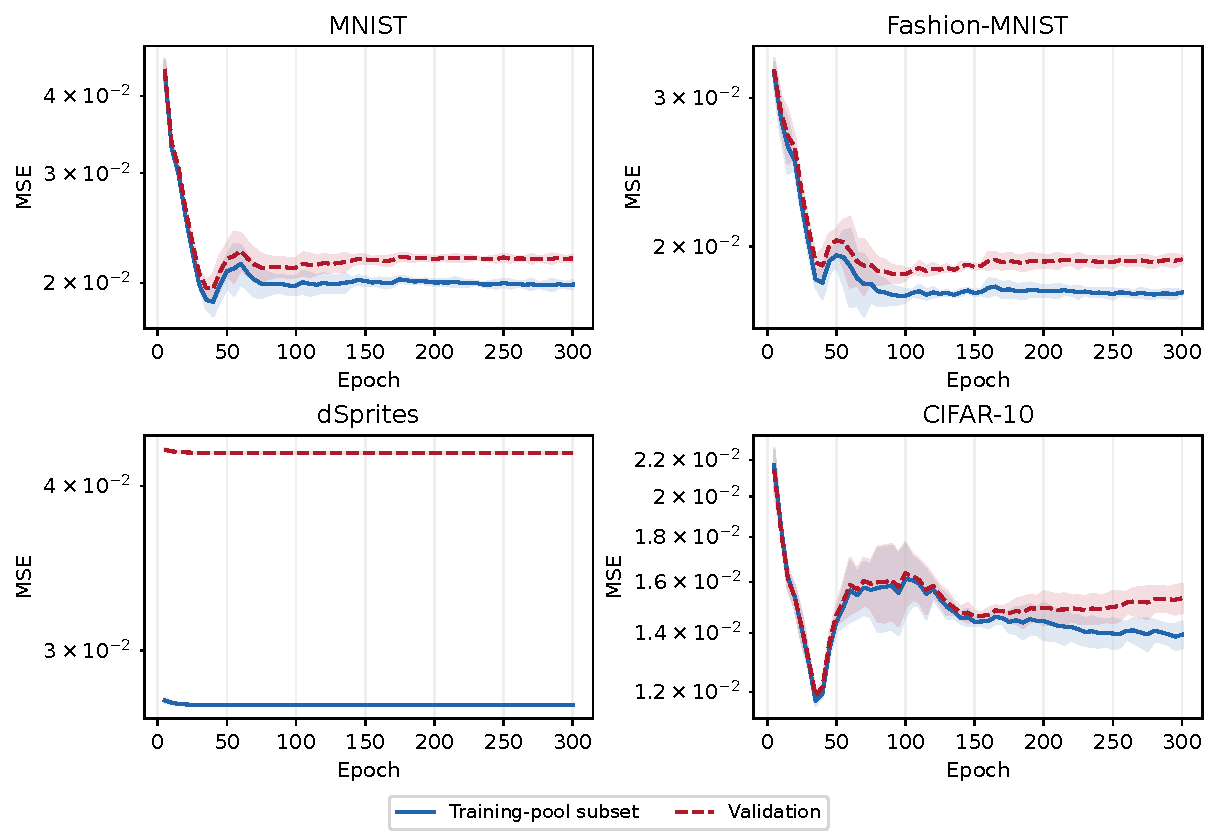
\includegraphics[width=\textwidth]{results/figures/MAKE52/arm_curves.pdf}
\caption{Native ARM posterior-mean MSE with the current binary gate mask,
evaluated every five epochs on a 2000-example training subset and the
validation split. Lines and shading are mean and sample SD over three
seeds. Vertical axes are logarithmic; a shaded lower bound is clipped
above zero for display. These curves do not reconstruct missing historical
ordinary-VAE training records.}
\label{fig:armcurves}
\end{figure}

\begin{figure}[!htbp]
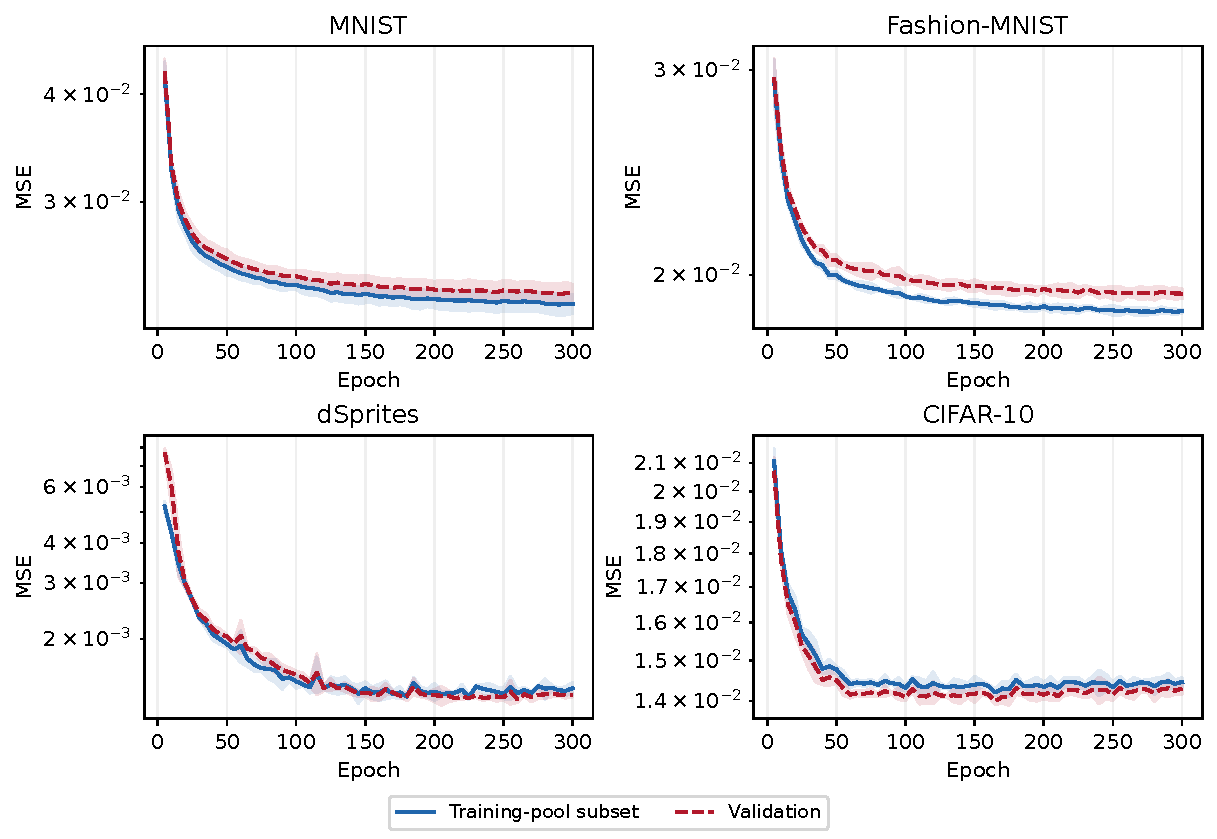
\includegraphics[width=\textwidth]{results/figures/MAKE52/ard_curves.pdf}
\caption{Full-width ARD posterior-mean MSE with zero-centre variance
updates, evaluated every five epochs. Mean and sample SD over three
seeds; logarithmic vertical axes. The 2000-example training-pool subset
includes 1800 examples reserved for prior updates and 200 used in
parameter-gradient training, so its curve is not a pure training-fit
estimate. No native pruning is applied in these evaluations.}
\label{fig:ardcurves}
\end{figure}

Table~\ref{tab:newtest} reports held-out test reconstruction at the
fixed final native models and transferred ordinary widths. Selection
uses the constraint or validation-based relevance readout, not these
test metrics. The full-model ARD column is deliberately distinguished
from quality at a selected native dimension.
@@table52:new_test@@

Table~\ref{tab:newcost} reports logged duration components. The source
records identify an NVIDIA GPU and the software environment. Training
intervals include periodic evaluation; the ARD initial and final prior
updates and final native evaluation are not included in the listed
training/Jacobian intervals. Jacobian timing pertains to 100 validation
examples and the particular architecture. Missing reference, anchor,
transfer and evaluation components preclude interpreting these numbers
as complete selector costs or combining them with historical CPU ID time.
@@table52:new_cost@@

The recorded \texttt{elbo} and \texttt{val\_elbo} fields remain in the
unmodified raw files for provenance but are not used as native ELBO
measurements (Section~\ref{sec:gpuvalidation}). Additional pruning
checkpoints were not saved, so native post-pruning ARD reconstruction
or a corrected native likelihood cannot be recovered from these
summary files alone. The analytic ARM-gradient check validates a
component; it cannot replace those model-level evaluations.
